\documentclass[convert={density=95,outext=.png}]{standalone}
\usepackage{tikz}
\usetikzlibrary{decorations.text}

\begin{document}

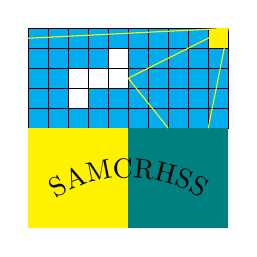
\begin{tikzpicture}[x = 1in, y = 1in]

\draw[fill = cyan] (0.0, 0.5) rectangle (0.1, 0.6);
\draw[fill = cyan] (0.0, 0.6) rectangle (0.1, 0.7);
\draw[fill = cyan] (0.0, 0.7) rectangle (0.1, 0.8);
\draw[fill = cyan] (0.0, 0.8) rectangle (0.1, 0.9);
\draw[fill = cyan] (0.0, 0.9) rectangle (0.1, 1.0);
\draw[fill = cyan] (0.1, 0.5) rectangle (0.2, 0.6);
\draw[fill = cyan] (0.1, 0.6) rectangle (0.2, 0.7);
\draw[fill = cyan] (0.1, 0.7) rectangle (0.2, 0.8);
\draw[fill = cyan] (0.1, 0.8) rectangle (0.2, 0.9);
\draw[fill = cyan] (0.1, 0.9) rectangle (0.2, 1.0);
\draw[fill = cyan] (0.2, 0.5) rectangle (0.3, 0.6);
\draw (0.2, 0.6) rectangle (0.3, 0.7);
\draw (0.2, 0.7) rectangle (0.3, 0.8);
\draw[fill = cyan] (0.2, 0.8) rectangle (0.3, 0.9);
\draw[fill = cyan] (0.2, 0.9) rectangle (0.3, 1.0);
\draw[fill = cyan] (0.3, 0.5) rectangle (0.4, 0.6);
\draw[fill = cyan] (0.3, 0.6) rectangle (0.4, 0.7);
\draw (0.3, 0.7) rectangle (0.4, 0.8);
\draw[fill = cyan] (0.3, 0.8) rectangle (0.4, 0.9);
\draw[fill = cyan] (0.3, 0.9) rectangle (0.4, 1.0);
\draw[fill = cyan] (0.4, 0.5) rectangle (0.5, 0.6);
\draw[fill = cyan] (0.4, 0.6) rectangle (0.5, 0.7);
\draw (0.4, 0.7) rectangle (0.5, 0.8);
\draw (0.4, 0.8) rectangle (0.5, 0.9);
\draw[fill = cyan] (0.4, 0.9) rectangle (0.5, 1.0);
\draw[fill = cyan] (0.5, 0.5) rectangle (0.6, 0.6);
\draw[fill = cyan] (0.5, 0.6) rectangle (0.6, 0.7);
\draw[fill = cyan] (0.5, 0.7) rectangle (0.6, 0.8);
\draw[fill = cyan] (0.5, 0.8) rectangle (0.6, 0.9);
\draw[fill = cyan] (0.5, 0.9) rectangle (0.6, 1.0);
\draw[fill = cyan] (0.6, 0.5) rectangle (0.7, 0.6);
\draw[fill = cyan] (0.6, 0.6) rectangle (0.7, 0.7);
\draw[fill = cyan] (0.6, 0.7) rectangle (0.7, 0.8);
\draw[fill = cyan] (0.6, 0.8) rectangle (0.7, 0.9);
\draw[fill = cyan] (0.6, 0.9) rectangle (0.7, 1.0);
\draw[fill = cyan] (0.7, 0.5) rectangle (0.8, 0.6);
\draw[fill = cyan] (0.7, 0.6) rectangle (0.8, 0.7);
\draw[fill = cyan] (0.7, 0.7) rectangle (0.8, 0.8);
\draw[fill = cyan] (0.7, 0.8) rectangle (0.8, 0.9);
\draw[fill = cyan] (0.7, 0.9) rectangle (0.8, 1.0);
\draw[fill = cyan] (0.8, 0.5) rectangle (0.9, 0.6);
\draw[fill = cyan] (0.8, 0.6) rectangle (0.9, 0.7);
\draw[fill = cyan] (0.8, 0.7) rectangle (0.9, 0.8);
\draw[fill = cyan] (0.8, 0.8) rectangle (0.9, 0.9);
\draw[fill = cyan] (0.8, 0.9) rectangle (0.9, 1.0);
\draw[fill = cyan] (0.9, 0.5) rectangle (1.0, 0.6);
\draw[fill = cyan] (0.9, 0.6) rectangle (1.0, 0.7);
\draw[fill = cyan] (0.9, 0.7) rectangle (1.0, 0.8);
\draw[fill = cyan] (0.9, 0.8) rectangle (1.0, 0.9);
\draw[fill = yellow] (0.9, 0.9) rectangle (1.0, 1.0);

\fill[color = yellow] (0.0, 0.0) rectangle (0.5, 0.5);
\fill[color = teal] (0.5, 0.0) rectangle (1.0, 0.5);

\draw[decoration={text along path, text = SAMCRHSS, text align = center},
      decorate] (0.0, 0.0) to[out=60, in=120] (1.0, 0.0);

\draw[color = yellow] (1.0, 1.0) -- (0.9, 0.5);
\draw[color = yellow] (1.0, 1.0) -- (0.5, 0.75) -- (0.7, 0.5);
\draw[color = yellow] (1.0, 1.0) -- (0.0, 0.95);

\end{tikzpicture}

\end{document}
